\scanpage{62}
% ll. 1–3, top and its right-hand gloss
\[
\begin{aligned}
\unsure{\beta_0|\beta_{\bullet}}:=\beta&=c\,\frac{\mu_0}{\overline{\mu}_1}
=c\,\frac{\lambda_0-1}{\overline{\lambda}_{\unsure{1|0}}-1}
=c\,\frac{(\lambda_0-1)(\lambda_1-1)}{(K_1-1)}
=\zeta(\lambda_0-1)(\lambda_1-1)\\
&\hspace{6cm}=\zeta\mu_0\mu_1
\end{aligned}
\]
\margin{$\deleted{\unsure{\xi}}\zeta=\dfrac{c}{K_1-1}\in\mathbb R$\\
$K_i=\operatorname{Tr}_{\mathbb C/\mathbb R}\lambda_i=\lambda_i+\overline{\lambda_i}$\\
$\hfill=\lambda_i+\lambda_i^{-1}$\\
$(\lambda_i\overline{\lambda_i}=1)$\\
\uline{NB} $\det\tau_0\tau_1=\lambda_0\lambda_1$\\
$\operatorname{Tr}\tau_0\unsure{t_1|\tau_1}=$}

% ll. 4–7
$\zeta$ satisfait à l'équation
\[
\frac{(\lambda_0-1)^2(\lambda_1-1)^2}{\lambda_0\lambda_1}
\left(\zeta^2+2\frac{\lambda_0+\lambda_1}{(\lambda_0-1)(\lambda_1-1)}\zeta
+\frac{\lambda_0^2+\lambda_1^2}{(\lambda_0-1)^2(\lambda_1-1)^2}\right)
=K\in\{-2,-1,0,\alpha,\alpha'\}
\]
qui exprime que $\tau_0^{C}\tau_1^C$ est d'ordre 2, 3, 4 ou 5.

$[u=\tau_0\tau_1$ a comme trace $\lambda_0+\lambda_1+\beta$, comme déterminant $\lambda_0\lambda_1]$, et $K=K(u)=\dfrac{(\operatorname{Tr}u)^2}{\det u}-2$

% ll. 8–10
\uline{NB} Si $\lambda=\exp i\theta$, $\lambda'=\exp i\theta'$, alors $\lvert\lambda+\lambda'\rvert=2\left|\cos\bigl(\frac{\theta'-\theta}{2}\bigr)\right|$, $\lvert\lambda^2+\lambda'{}^2\rvert=2\unsure{\cos|\lvert\cos}(\theta'-\theta)$
\[
\begin{aligned}
|\lambda-1|^2&=2-K(\lambda)\qquad K(\lambda)=\operatorname{Tr}_{\mathbb C/\mathbb R}\lambda=2\cos\theta\\
|\lambda-1|&=2\left|\sin\frac{\theta}{2}\right|
\end{aligned}
\]

% ll. 11–12
\[
\left\{\begin{aligned}
2\frac{\lambda+\lambda'}{(\lambda-1)(\lambda'-1)}
&=-\frac{\deleted{4}\cos\frac{\theta'-\theta}{2}}{\deleted{4}\sin\frac\theta2\sin\frac{\theta'}2}\\
\deleted{\unsure{2}}\frac{\lambda_{\unsure{0}}^2+\lambda'{}^2}{(\lambda-1)^2(\lambda'-1)^2}
&=\frac{2\cos(\theta'-\theta)}{16\sin^2\frac\theta2\sin^2\frac{\theta'}2}
=\frac{1}{\deleted{\unsure{4}}8}\frac{\cos(\theta'-\theta)}{\sin^2\frac\theta2\sin^2\frac{\theta'}2}
\end{aligned}\right.
\]
\margin{$\dfrac{(\lambda_0-1)^2(\lambda_1-1)^2}{\lambda_0\lambda_1}=16\sin^2\!\frac{\theta_0}2\sin^2\!\frac{\theta_1}2$\\
$0<\theta_0,\theta_1\leq\pi$}

% ll. 13–16
\[
\begin{aligned}
\zeta^2&-\frac{\cos\frac{\theta_1-\theta_0}2}{\sin\frac{\theta_0}2\sin\frac{\theta_1}2}\zeta+
\frac{1}{\deleted{\unsure{8}}16}\left(
\frac{\deleted{\unsure{2}}2\cos(\theta_1-\theta_0)-K}
{\sin^2\frac{\theta_0}2\sin^2\frac{\theta_1}2}
\deleted{\unsure{-\frac{K}{16\sin^2\frac{\theta_0}2\sin^2\frac{\theta_1}2}}}\right)=0\\
\Delta(K)&=\frac12\frac{\deleted{\cos\frac{\theta_1-\theta_0}2}}{\sin^2\frac{\theta_0}2\sin^2\frac{\theta_1}2}
\left[\underbrace{2\cos^2\frac{\theta_1-\theta_0}2-\cos\left(\frac{\theta_1-\theta_0}{\deleted{\unsure{2}}}\right)}_{1}+
\frac{\deleted{\unsure{2}}1}{2}K\right]\\
&=\deleted{\unsure{\frac{2+K/2}{2\sin^2\frac{\theta_0}2\sin^2\frac{\theta_1}2}}}
=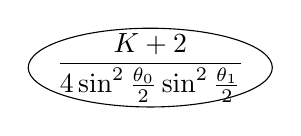
\begin{tikzpicture}[baseline=(x.base)]\node[inner sep=1pt](x){$\displaystyle\frac{K+2}{4\sin^2\frac{\theta_0}2\sin^2\frac{\theta_1}2}$};\draw (x.center) ellipse (1.55cm and .50cm);\end{tikzpicture}
=\ \geqslant0\\
&\hspace{6cm}=\frac{\cos^2\frac\theta2}{\sin^2\frac{\theta_0}2\sin^2\frac{\theta_1}2}
\end{aligned}
\]
\margin{$K+2=2(1+\cos\theta)$\\ $=4\cos^2\frac{\theta}{2}$}
% margin note written sideways
\margin{\rotatebox{90}{\scriptsize $\displaystyle
\zeta=\frac12\left[\frac{\cos\frac{\theta_1-\theta_0}2}{\sin\frac{\theta_0}2\sin\frac{\theta_1}2}
\pm\frac{\deleted{\unsure{\sqrt{K+2}}}\cos\frac\theta2}{\deleted{2}\sin\frac{\theta_0}2\sin\frac{\theta_1}2}\right]
=\frac{1}{\unsure{2}\sin\frac{\theta_0}2\sin\frac{\theta_1}2}
\left[\deleted{\unsure{2}}\cos\frac{\theta_1-\theta_0}2\pm
\deleted{\unsure{\sqrt{K+2}}}\cos\frac\theta2\right]$}}

% ll. 17–20
\deleted{\unsure{Alors} \illegible{2} $\unsure{K+2}$ \unsure{jamais nul} $(\unsure{K+2-\frac18K})$}

N'est nul que si $K=-2$ i.e. $\tau_0^C\tau_1^C$ est d'ordre 2. auquel cas l'unique solution est
\[
\boxed{\zeta=\frac{\cos\frac{\theta_1-\theta_0}2}{2\sin\frac{\theta_0}2\sin\frac{\theta_1}2}}
\]
suivant les valeurs de $\lambda_i=\exp 2i\pi/\nu_i$\quad $2\leq\nu_i\leq5$

Ceci fait $\deleted{16}\inserted{=15}$ possibilités. (en excluant $\nu_0=\nu_1=2$)
% archive sheet number: 61
